\documentclass[a4paper, 11pt]{article}
\usepackage{multirow}
\usepackage{soul}
\usepackage{graphicx}
\usepackage{amsmath}
\usepackage[export]{adjustbox}
\usepackage{float}
\usepackage[margin=1in]{geometry}
\usepackage{gensymb}
\usepackage{listings}
\usepackage{indentfirst}
\usepackage{xcolor}
% \usepackage[draft,nosingleletter]{impnattypo}

\usepackage{xcolor}

\definecolor{codegreen}{rgb}{0,0.6,0}
\definecolor{codegray}{rgb}{0.5,0.5,0.5}
\definecolor{codepurple}{rgb}{0.58,0,0.82}
\definecolor{backcolour}{rgb}{0.95,0.95,0.92}

\lstdefinestyle{mystyle}{
    backgroundcolor=\color{backcolour},   
    commentstyle=\color{codegreen},
    keywordstyle=\color{blue},
    numberstyle=\tiny\color{codegray},
    stringstyle=\color{codepurple},
    basicstyle=\ttfamily\footnotesize,
    breakatwhitespace=false,         
    breaklines=true,                 
    captionpos=b,                    
    keepspaces=true,                 
    numbers=left,                    
    numbersep=5pt,                  
    showspaces=false,                
    showstringspaces=false,
    showtabs=false,                  
    tabsize=2
}

\lstset{style=mystyle}

\begin{document}

\begin{center}
	\begin{tabular}{cc}
		\hline
		\multicolumn{2}{|c|}{\begin{tabular}[c]{@{}c@{}} \\ \LARGE \so{Informatyka w Medycynie - Laboratorium} \\ \\ \end{tabular}}         \\ \hline
		\multicolumn{2}{|c|}{\begin{tabular}[l]{@{}l@{}}\\\Large Tomografia komputerowa - projekt \\ \\ \end{tabular}}                      \\ \hline
		\multicolumn{1}{|l|}{\begin{tabular}[l]{@{}l@{}} \\ \hspace{2cm}Kierunek/semestr: Informatyka/6 \hspace{2cm} \\ \\ \end{tabular}} &
		\multicolumn{1}{|c|}{\begin{tabular}[l]{@{}l@{}} \\ Grupa: L16 \\ \\ \end{tabular}}                                                 \\ \hline
		\multicolumn{2}{|c|}{\begin{tabular}[c]{@{}c@{}}\\ Jakub Kwiatkowski 145356 \\Paweł Strzelczyk 145217  \\ \\ \end{tabular}}         \\ \hline
	\end{tabular}
\end{center}

\section{Opis projektu.}

Projekt został przygotowany w formie interaktywnego notatnika Jupyter Notebook.

Symulowany tomograf jest tomografem typu stożkowego (fan-beam CT scanner).

Do wykonania symulacji wykorzystano język Python 3 oraz biblioteki

\begin{itemize}
	\item numpy
	\item matplotlib
	\item skimage
	\item OpenCV
	\item Pydicom
	\item ipython (ipywidgets, IPython)
\end{itemize}

\section{Opis głównych funkcji programu.}

\subsection{Pozyskiwanie odczytów dla poszczególnych detektorów.}

Aby pozyskać odczyty trzeba najpierw ustalić pozycję emitera oraz detektorów.\\
Mając obraz o wymiarach $m \times n$ oraz położenie kątowe emitera $\alpha$
możemy wyliczyć pozycję emitera na okręgu opisanym na obrazie:
\begin{align*}
	 & radius = \sqrt{\frac{m^2}{2^2} + \frac{n^2}{2^2}} \\
	 & emitter_x = \cos\alpha * radius + \frac{m}{2}     \\
	 & emitter_y = \sin\alpha * radius + \frac{n}{2}     \\
\end{align*}

\newpage

Znając dodatkowo rozpiętość kątową wachlarza detektorów $\phi$ oraz ich liczbę $D$ możemy obliczyć pozycję każdego z nich:

\begin{align*}
	 & step = \frac{\phi}{D - 1}             \\
	 & start = \alpha + \pi - \frac{\phi}{2} \\
	 & \forall_{i \in D}
	\begin{cases}
		detector^{i}_{x} = \cos(start + i * step) * radius + \frac{m}{2} \\
		detector^{i}_{y} = \sin(start + i * step) * radius + \frac{n}{2}
	\end{cases}
\end{align*}

Translacja o $\frac{m}{2}$ i $\frac{n}{2}$ wynika z faktu, że punkt centralny obrazu nie leży w środku układu współrzędnych.


Po wyznaczeniu współrzędnych emitera i detektorów, dla każdej pary emiter -- detektor wyznaczamy piksele
przez które przechodzi odcinek łączący tę parę (wykorzystujemy tu funkcję line\_nd [listing \ref{lst:sinogram}] z pakietu scikit-image)
i sumujemy wartości tych pikseli, dzięki czemu otrzymujemy sinogram obrazu.

\begin{lstlisting}[language = Python, caption = Wyliczanie sinogramu, label = lst:sinogram]
	def detector_positions(alpha, phi, count, shape):
    """
    Calculates locations of detectors in a fan-beam CT scanner.

    :param alpha: Emitter's angular position angle (in radians).
    :param phi: Detectors' angular span (in radians) [measured from circle's center].
    :param count: Number of detectors.
    :param shape: Image size (x, y).
    :return: List of detector positions (x, y).    
    """

    from numpy import pi as PI, cos, sin, sqrt, round, int64

    w, h = shape
    radius = round(sqrt(w ** 2 + h ** 2) / 2).astype(int64)

    angular_step = phi / (count - 1)
    start_angle = alpha + PI - (phi / 2)

    x = lambda index: round(cos(start_angle + angular_step * index) * radius).astype(int64) + (w // 2)
    y = lambda index: round(sin(start_angle + angular_step * index) * radius).astype(int64) + (h // 2)

    return [(x(no), y(no)) for no in range(count)]


def emitter_position(alpha, shape]) -> list[tuple[int, int]]:
    """
    Calculates emitter's location in a fan-beam CT scanner.

    :param alpha: Emitter's angular position (in radians).
    :param shape: Image size (x, y).
    :return: Emitter's position (x, y).
    """

    from numpy import cos, sin, sqrt, round, int64

    w, h = shape
    radius = round(sqrt(w ** 2 + h ** 2) / 2).astype(int64)

    x = round(cos(alpha) * radius).astype(int64) + (w // 2)
    y = round(sin(alpha) * radius).astype(int64) + (h // 2)

    return (x, y)

def scanlines(bounds, emitter, detectors):
	"""
	Calculates scanlines (pixels in ray path) for a CT scanner.

	:param bounds: Image's bounds (x, y).
	:param emitter: Emitter's position (x, y).
	:param detectors: List of detector positions (x, y).

	:return: List of scanlines (list of lists of pixels in ray path (one for every detector)).

	This function automatically removes pixels not in the image's bounds.
	"""

	from skimage.draw import line_nd

	w, h = bounds

	in_bounds = lambda point: point[0] >= 0 and point[0] < w and point[1] >= 0 and point[1] < h

	ex, ey = emitter

	# line_nd uses transposed coordinates (y, x), so we need to swap them.
	lines = [list(filter(in_bounds, zip(*line_nd((d[1], d[0]), (ey, ex))))) for d in detectors]

	return [[x for x in zip(*line)] for line in lines]


from numpy import ndarray


def radon_for(image, alpha, phi, count):
	"""
	Calculates Radon transform of an image for given alpha angle.

	:param alpha: Emitter's angular position (in radians)
	:param phi: Detectors' angular span [measured from circle's center] (in radians).
	:param count: Number of detectors.
	"""

	from numpy import sum

	w, h = image.shape[:2]

	emitters = emitter_position(alpha, (w, h))
	detectors = detector_positions(alpha, phi, count, (w, h))
	lines = scanlines((w, h), emitters, detectors)

	row = []
	for line in lines:
	if len(line) == 0:
	row.append(0)
	continue
	r, c = line
	row.append(sum(image[r, c]))

	return row


def radon(image, phi, step, count) -> ndarray:
	"""
	Calculates Radon transform of an image for given alpha angle.

	:param phi: Detectors' angular span [measured from circle's center] (in degrees).
	:param step: Step size (in degrees).
	:param count: Number of detectors.
	"""

	from numpy import deg2rad, arange, array, pi

	phi = deg2rad(phi)
	step = deg2rad(step)

	sinogram = []

	for angle in arange(0, pi * 2, step):
	sinogram.append([angle] + radon_for(image, angle, phi, count))

	return array(sinogram)
\end{lstlisting}

\subsection{Filtrowanie sinogramu.}

Wykorzystane filtrowanie jest prostym splotem nazwanym filtrem medianowym.


Aby obraz nie został zbytnio rozmyty zastosowaliśmy jądro o wymiarach $3\times3$  piksele.

\subsection{Ustalanie jasności poszczególnych punktów obrazu wynikowego oraz jego przetwarzanie końcowe.}

Po wykonaniu odwrotnej transformacji Radona za pomocą techniki \textit{back-projection} otrzymany obraz zawiera piksele o
jasnościach wykraczających poza ramy kanału 8-bitowego, dlatego obraz musi zostać znormalizowany.\\


Normalizacja transformuje obraz z nieograniczonej prawostronnie reprezentacji całkowitoliczbowej do reprezentacji
zmiennoprzecinkowej w zakresie $\left[0.0;1.0\right]$. Normalizacja przebiega według schematu:

\begin{align*}
	\forall_{p \in P(x, y)} p' = \frac{p - \min(P)}{\max(P) - \min(P)}
\end{align*}

\subsection{Wyznaczanie wartości miary RMSE.}

Miara RMSE jest obliczana poprzez wyliczenie odchylenia standardowego różnicy obrazów -- wejściowego i wyjściowego.

\subsection{Odczyt i zapis plików DICOM.}

Do obsługi standardu DICOM wykorzystano bibliotekę Pydicom.\\
\\
Dla uproszczenia odczytu i zapisu stworzone zostały funkcje pomocnicze przedstawione na listingu \ref{lst:dicom}.

\begin{lstlisting}[language = Python, caption = Obsługa DICOM, label = lst:dicom]
def read_from_dicom(filename) -> ndarray:
    """
    Reads pixel data from DICOM file and returns it as ndarray.

    WARNING: Currently this function assumes that image is single and in grayscale.
    !!! COLOR & MULTIPLANAR IMAGES ARE NOT SUPPORTED !!!
    """

    from pydicom import dcmread

    contents = dcmread(filename)

    return contents.pixel_array


def write_to_dicom(filename, image: ndarray, data: dict):
    """
    Writes data to DICOM file.

    :param image: image data in form of ndarray.
    WARNING: Currently this function assumes that image is single and in grayscale.
    !!! COLOR & MULTIPLANAR IMAGES ARE NOT SUPPORTED !!!

    :param data: Dictionary with keys "id", "name", "date", "comments" 
    """
    from skimage.util import img_as_ubyte
    from pydicom.uid import generate_uid, ExplicitVRLittleEndian
    from pydicom._storage_sopclass_uids import CTImageStorage
    from pydicom.dataset import validate_file_meta
    from pydicom import Dataset, FileDataset

    image = img_as_ubyte(image)

    # Populate required values for file meta information
    meta = Dataset()
    meta.MediaStorageSOPClassUID = CTImageStorage
    meta.MediaStorageSOPInstanceUID = generate_uid()
    meta.TransferSyntaxUID = ExplicitVRLittleEndian

    ds = FileDataset(None, {}, preamble = b"\0" * 128)
    ds.file_meta = meta

    ds.is_little_endian = True
    ds.is_implicit_VR = False

    ds.SOPClassUID = CTImageStorage
    ds.SOPInstanceUID = meta.MediaStorageSOPInstanceUID

    ds.PatientID = data["id"]
    ds.PatientName = data["name"]
    ds.StudyDate = data["date"]
    ds.ImageComments = data["comments"]

    ds.Modality = "CT"
    ds.SeriesInstanceUID = generate_uid()
    ds.StudyInstanceUID = generate_uid()
    ds.FrameOfReferenceUID = generate_uid()

    ds.BitsStored = 8
    ds.BitsAllocated = 8
    ds.SamplesPerPixel = 1
    ds.HighBit = 7

    ds.ImagesInAcquisition = 1
    ds.InstanceNumber = 1

    ds.Rows, ds.Columns = image.shape

    ds.ImageType = r"ORIGINAL\PRIMARY\AXIAL"

    ds.PhotometricInterpretation = "MONOCHROME2"
    ds.PixelRepresentation = 0

    validate_file_meta(ds.file_meta, enforce_standard = True)

    ds.PixelData = image.tobytes()

    ds.save_as(filename, write_like_original = False)
\end{lstlisting}


\section{Wpływ poszczególnych parametrów na jakość obrazu wynikowego.}
\subsection{Liczba detektorów.}

Liczba detektorów jest zmieniana w przedziale $\left<90, 720 \right>$ z krokiem $90$.

\begin{center}
	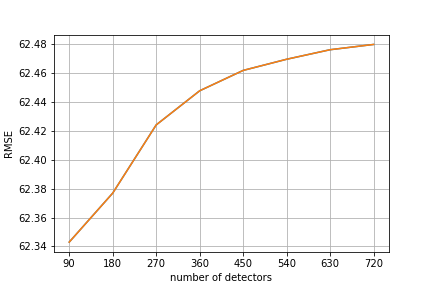
\includegraphics[width=0.7\textwidth]{detectors.png}
\end{center}
\subsection{Liczba skanów.}

Liczba skanów jest zmieniana w przedziale $\left<90, 720 \right>$ z krokiem $90$.

\begin{center}
	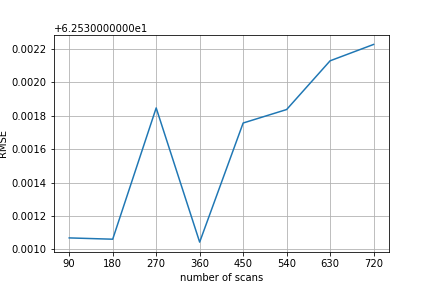
\includegraphics[width=0.7\textwidth]{scans.png}
\end{center}
\subsection{Rozpiętość wachlarza.}

Rozpiętość wachlarza jest zmieniana w przedziale $\left<45, 270 \right>$ z krokiem $45$.

\begin{center}
	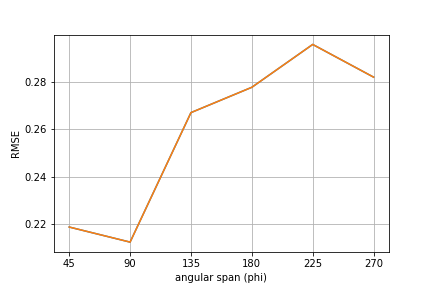
\includegraphics[width=0.7\textwidth]{phi.png}
\end{center}
\subsection{Filtr splotowy.}
\begin{center}
	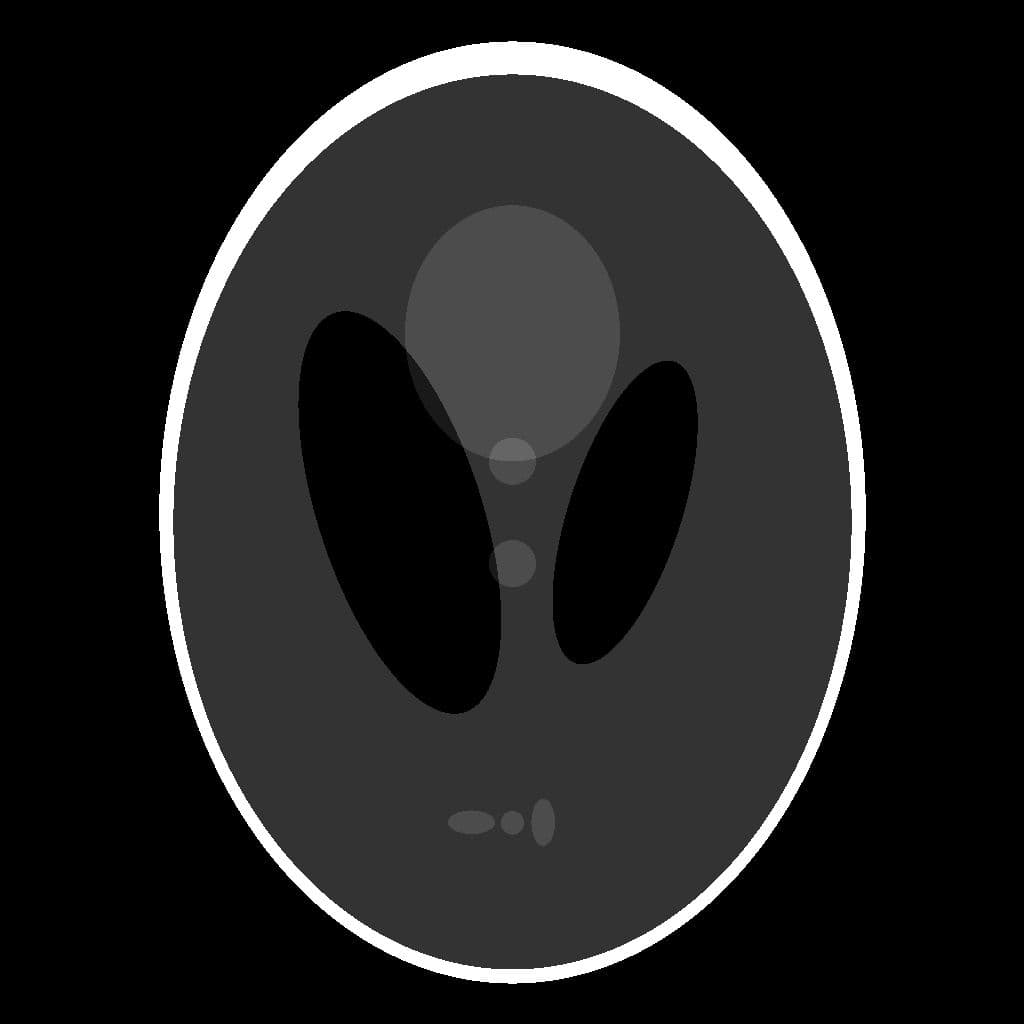
\includegraphics[width=0.8\textwidth]{phantom.png}


	Obraz testowy do obliczeń z wykorzystaniem filtra.
\end{center}

\begin{center}
	Rekonstrukcja bez filtrowania.


	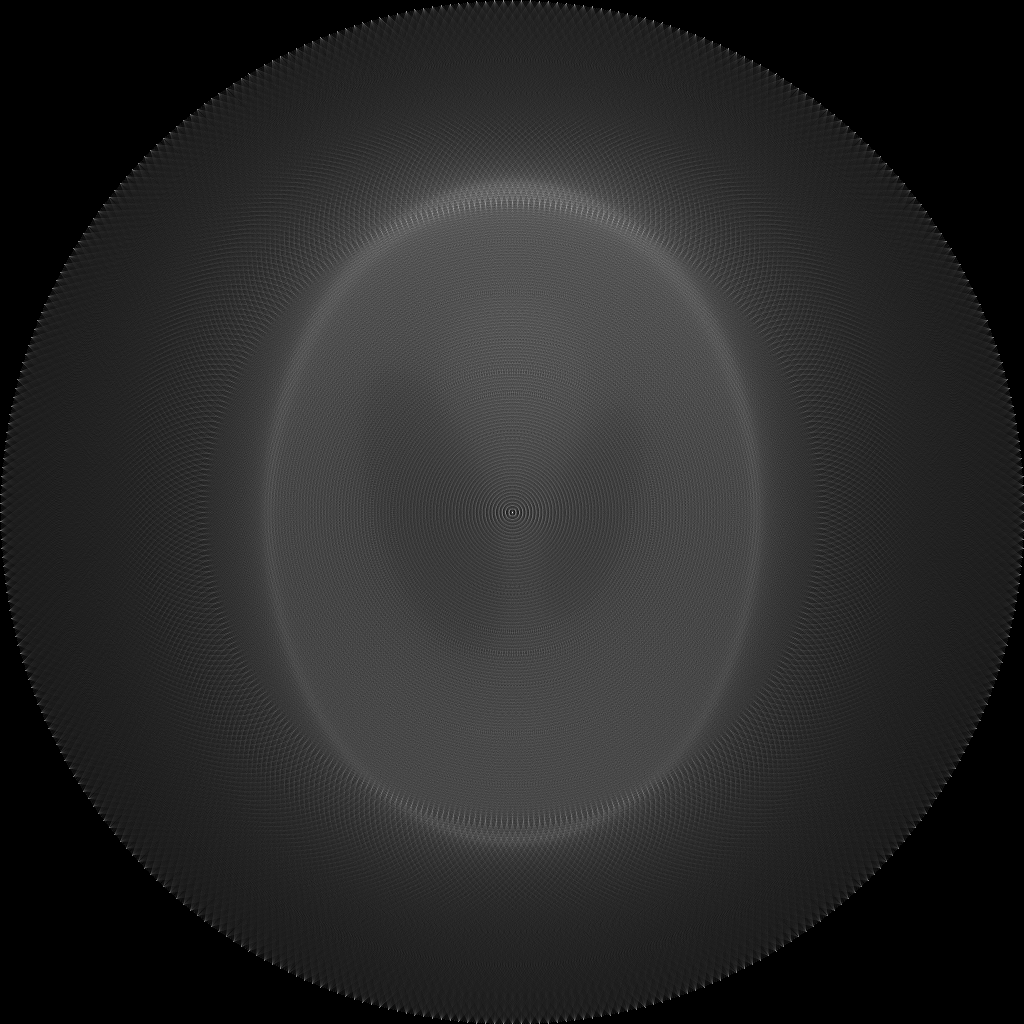
\includegraphics[width=0.4\textwidth]{reconstructed1.png}
	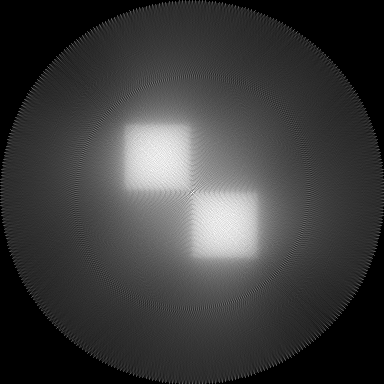
\includegraphics[width=0.4\textwidth]{reconstructed2.png}

	RMSE1 0,20693420547948 \hspace{1.5cm} RMSE2 0,266156126913852

\end{center}


\begin{center}
	Rekonstrukcja z filtrem.


	
\includegraphics[width=0.4\textwidth]{reconstructed_filtered1.png}
	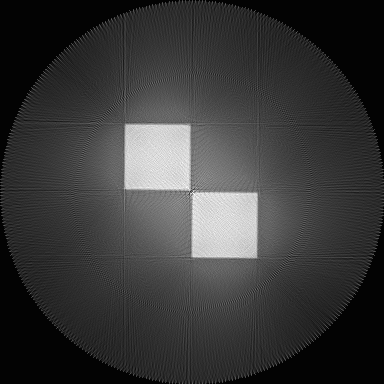
\includegraphics[width=0.4\textwidth]{reconstructed_filtered2.png}

	RMSE1 filtr - 0,249729691096470\hspace{1.5cm} RMSE2 filtr - 0,26778570956508
\end{center}

\section{Zmiana RMSE podczas wykonywania kolejnych iteracji odwrotnej transformaty Radona.}


Parametry transformacji:
\begin{itemize}
	\item liczba detektorów - 180
	\item rozpiętość wachlarza - 180\degree
	\item łączna liczba skanów - 180
\end{itemize}
\begin{center}
	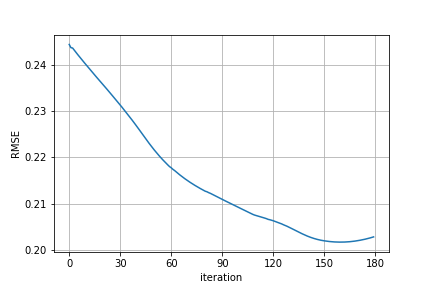
\includegraphics[width=0.7\textwidth]{change.png}
\end{center}
\end{document}